\section{Other Features}\label{otherFeatures}

%%
\subsection{AutoBackup and Recovery}\label{autoBackup}

Temporary backups of open projects are generated every minute for
projects which have previously been saved to disk (new projects not yet
saved are not backed up). If Blue quits unexpectedly, those files will
remain, otherwise on normal closing of the file they are deleted. If on
opening a file a backup if found with a date newer than the original
file, the option to open from the backup or the original is given.

If the backup is chosen, it is required to use "Save As" to save over
the original file or to a new file. At that point the backup is deleted.

If the original file is chosen, then the backup file will be overwritten
the next time the autobackup thread runs.

%%
\subsection{Sound Object Freezing}\label{soundObjectFreezing}

Sound Object Freezing allows you to free up CPU-cycles by pre-rendering
soundObjects. Frozen soundObjects can work with global processing
instruments, and files are relative to the directory the project file is
in, so can be moved from computer to computer without problem. Frozen
soundObjects can be unfrozen at anytime, returning the original
soundObject and removing the frozen wave file.

To freeze a soundObject, select one or many soundObjects on the
timeline, rt-click on a selected soundObject, and then select
"Freeze/Unfreeze SoundObjects". To unfreeze, select one or many frozen
soundObjects and select the same menu option.

On the timeline, if your soundObject rendered wave is longer in duration
than the original soundObject's duration (as is the case if you have
reverb processing), the frozen soundObject's bar will graphically show
the difference in times with two different colors.

Note: As currently implemented, when Blue goes to freeze soundObjects it
may appear to be frozen, but messages will continue to appear in the
console showing that csound is rendering the frozen soundObjects. Future
versions will be more polished.

\begin{enumerate}
\def\labelenumi{\arabic{enumi}.}
\item
  An soundObject is selected
\item
  Using the same project settings (all of the instruments, tables,global
  orc/sco, etc.) but not scoreTimeline generated sco, Blue generates the
  sco for the selected soundObject and produce a temporary .csd file
\item
  Blue runs csound with "csound -Wdo freezex.wav tempfile.csd" where the
  x in freezex.wav is an integer, counting up. This wav file is
  generated in the same directory that the projectFile is located.
\item
  Blue replaces the soundObject in the timeline with a
  FrozenSoundObject. The FrozenSoundObject keeps a copy of the original
  soundObject (for unfreezing), as well as shows the name of the frozen
  wav file, the original soundObject's duration, and the frozen wav
  file's duration (not necessarily the same, as is the case if using
  global reverb, for example).
\item
  When you do a render of the entire piece now, the frozen sound object
  generates a very simple wav playing csound instrument that will play
  the rendered wav file as-is. The instrument looks something like:

\begin{verbatim}
aout1, aout2    diskin    p4         
                outs      aout1, aout2 
          
\end{verbatim}

  and the FrozenSoundObject only generates a single note that has the
  start-time, the duration of the frozen wav file, and the name of the
  file. This will end up playing the soundFile exactly as if the SCO for
  the original soundObject was generated. This also bypasses any routing
  to global sound processing, as if you had any of these effects
  originally, the would be generated as part of the frozen file.
\end{enumerate}

\begin{itemize}
\item
  You can select multiple soundObjects and batch freeze and unfreeze
  -the generated wav file may be longer than the original soundObject,
  due to global processing instruments (like reverb, echo, etc.) This is
  taken into account.
\item
  The freezing system does *not* work for all graph toplogies. If you're
  using soundObjects with instruments used as control signals, this
  won't work unless the notes for the instruments they are controlling
  are alsoin the same soundObject. I.e. I have one soundObject that has
  only notes that affect global variables, while I have one instrument
  thatuses those global variables. This could work though if you
  repackage the set of soundObjects into a polyObject. Probably best to
  generalize as:

  \begin{itemize}
  \item
    Your soundObject must be self-contained
  \item
    All sound output from instruments go directly out or piped through
    always-on instruments, that most likely should take advantage of the
    \textless{}total\_dur\textgreater{} variable, as well as the new
    \textless{}processing\_start\textgreater{} variable (more about this
    when I release, but together with freezing, this lets you set the
    start time of always-on instruments to the first time where
    non-frozen soundObjects occur, so if the first half of your piece is
    frozen and you're unfrozen stuff is in the second half, you don't
    need always on instruments to be turned on until the second half as
    the first half is routed to outs
  \end{itemize}
\item
  This system is tested with 2-channel pieces. I'm not sure if this will
  work with higher number of channels, but I don't see why it wouldn't.
\item
  Changing the number of channels on the project after a freeze may
  cause Csound errors when rendering the frozen soundObject (can be
  remedied by unfreezing and refreezing)
\item
  Frozen files are referenced relatively to the project file, so you are
  free to move your project directory around or rename it and the frozen
  files will work fine.
\end{itemize}


\subsection{Importing ORC/SCO and CSD Files}\label{importCSD}

Blue is able to import ORC/SCO and CSD files and set up a Blue project
file, with instruments parsed out and put into the orchestra manager,
project settings set, etc. Currently, there are three options to choose
from when importing a CSD file, all relating to how you would like to
import the notes from the CsScore section:

\begin{itemize}
\item
  Import Score to Global Score - all score goes to the Global Score
  section
\item
  Import All Score to Single SoundObject - all score goes into a single
  GenericScore SoundObject. The duration of the soundObject will be set
  to the duration of the imported score. This is broken up into
  different soundObjects and layers if sections (s-statement) are found
  in the score.
\item
  Import Score and Split into SoundObjects by Instrument Number - score
  is split by instrument number and a different GenericScore soundObject
  will be created for each block of score text per instrument. This is
  broken up into different soundObjects and layers if sections
  (s-statement) are found in the score.
\end{itemize}

\begin{itemize}
\item
  From the CsScore, Blue will only import f-, i-, and s- statements.
  Other score statements are not currently supported at this time.
\end{itemize}

%%
\subsection{Importing MIDI Files}\label{importMIDI}

Blue is able to import MIDI files and set up a Blue project file from
the note information in the MIDI file, using the settings given by the
user. To import a MIDI file, choose the "Import MIDI File" option from
the File menu. Next, using the file dialog to locate the MIDI file to
import. After selecting the desired file, Blue will show the following
MIDI Import Settings dialog for you to configure how you would like to
import the MIDI note information. (Note: Blue will only show information
for tracks where note data was found.)

MIDI Import Settings

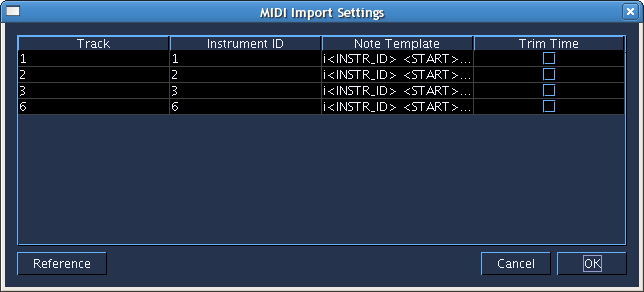
\includegraphics{images/midiImportSettings.png}

The table column information is as follows:

\begin{description}
\item[Track]
The original MIDI track number to which this setting is to be applied
to. This column is not editable is for reference purpose only.
\item[Instrument ID]
The Csound instrument ID to use for this track. This will replace the
\textless{}INSTR\_ID\textgreater{} key within the note template. This
value is treated as a string to allow users to assign the track
information to Csound named instruments. If one is doing so, one must
quote the name, i.e. use "trumpet" instead of trumpet (without quotes),
otherwise the output will not be legal Csound SCO. Default value is the
number of the MIDI track.
\item[Note Template]
Template note text to use for generating Csound SCO from the MIDI data.
The default note template is "i\textless{}INSTR\_ID\textgreater{}
\textless{}START\textgreater{} \textless{}DUR\textgreater{}
\textless{}KEY\textgreater{} \textless{}VELOCITY\textgreater{}". By
having note templates, the user can massage the note information to work
with any number of pfields that their instruments require.

The following values are allowed in the note template:

\begin{longtable}[]{@{}ll@{}}
\caption{Key Values}\tabularnewline
\toprule
Shortcuts & Description\tabularnewline
\midrule
\endfirsthead
\toprule
Shortcuts & Description\tabularnewline
\midrule
\endhead
\textless{}INSTR\_ID\textgreater{} & The instrument ID assigned in the
track settings.\tabularnewline
\textless{}START\textgreater{} & Start Time of Note\tabularnewline
\textless{}DUR\textgreater{} & Duration of Note\tabularnewline
\textless{}KEY\textgreater{} & MIDI key number\tabularnewline
\textless{}KEY\_PCH\textgreater{} & MIDI key number as Csound
PCH\tabularnewline
\textless{}KEY\_OCT\textgreater{} & MIDI key number as Csound
OCT\tabularnewline
\textless{}KEY\_CPS\textgreater{} & MIDI key number as
CPS\tabularnewline
\textless{}VELOCITY\textgreater{} & MIDI velocity number\tabularnewline
\textless{}VELOCITY\_AMP\textgreater{} & MIDI velocity number as
amplitude\tabularnewline
\bottomrule
\end{longtable}

The button labelled "Reference" on the dialog will pop open the above
information for quick reference of the allowable replacement keys for
note templates.
\item[Trim Time]
This option will shift the generated SoundObject to the time of the
first note and then take the generated notes for the track and shift
them all so that the first note starts at time 0 so that there is no
empty time at the beginning of the track's note information.
\end{description}

After finishing configuring settings for the imported MIDI data, Blue
will generate the notes with one SoundLayer per MIDI track, and on each
SoundLayer it will contain one GenericScore SoundObject containing the
converted MIDI score.

\begin{quote}
\textbf{Note}

The current implementation does not handle cases where there are
overlapping notes of the same MIDI note number within the same track and
results are unpredictable. Also, only MIDI files where time is PPQ is
supported at the moment (non-SMPTE). Users wanting support for either of
these cases or have other ideas they would like implemented are
requested to make feature requests on the Blue mailing list or to use
the help menu "Request a Feature" option.
\end{quote}

%%
\subsection{Blue Variables}\label{blueVariables}

Blue treats special text as special Blue variables. Below is a list of
those variables.

\begin{longtable}[]{@{}ll@{}}
\toprule
Variable & Value\tabularnewline
\midrule
\endhead
\textless{}TOTAL\_DUR\textgreater{} & Duration of the generated score
from the timeline (Available in Global SCO text area.)\tabularnewline
\textless{}INSTR\_ID\textgreater{} & Replaces with instrumentId; if the
instrument is a named instrument, value is quoted. Generally used when
creating notes.(Available within instruments and some
SoundObjects.)\tabularnewline
\textless{}INSTR\_NAME\textgreater{} & Replaces with instrumentId; if
the instrument is a named instrument, the value is not quoted. Generally
used when working with ORC code to give a variable a unique ID, i.e.
"gk\_var\textless{}INSTR\_NAME\textgreater{}".(Available within
instruments and some SoundObjects.)\tabularnewline
\textless{}RENDER\_START\textgreater{} & The start time of rendering.
Does not take into account time warping of score. (Available in Global
SCO text area.)\tabularnewline
\textless{}RENDER\_START\_ABSOLUTE\textgreater{} & The start time of
rendering. Takes into account time warping of score. (Available in
Global SCO text area.)\tabularnewline
\textless{}PROCESSING\_START\textgreater{} & The time value when
always-on effects instruments need to start. Calculated as the time
value of the first soundObject that is not a FrozenSoundObject or
Comment. (Available in Global SCO text area.)\tabularnewline
\bottomrule
\end{longtable}

%%
\subsection{Command Line Options for Blue}\label{commandLine}

To view the options that Blue has from the commandline, type "blue
-\/-help". After that, you should see information printed to the
console. Some of these flags are used by the Netbeans Platform that Blue
is built upon. The following are ones Blue uses itself:

\begin{verbatim}
  -c, --compile <arg>       
  -o, --output <arg>
\end{verbatim}

The flags above allow for commandline compilation of a .blue project
into a CSD. Both flags must be set to work. An example of usage is:

\begin{verbatim}
blue -csomeFile.blue -ooutput.csd
\end{verbatim}

This will use somefile.blue and produce output.csd. The generated CSD
will use the Disk Render settings for the project. Using the commandline
option for compiling .blue projects is useful for automating builds of
projects using a build system like Make, Rake, Ant, or other tool.
